% Mechanical Design Report - Sensor Box Housing
\documentclass[12pt]{article}
\usepackage[margin=1in]{geometry}
\usepackage{graphicx}
\usepackage{caption}
\usepackage{float}

\title{Mechanical Design Report\\Sensor Box Housing}
\author{0104C}
\date{\today}

\begin{document}

\maketitle

\section{Introduction}

This report documents the mechanical design process for the sensor box, the enclosure that houses the electronic components and serves as the physical interface for the deployment system. The process covers the initial box concept, the decision to use a slidable lid, and the outcome of the first 3D print attempt.

\section{Design Process}

\subsection{Initial Box Concept}

The sensor box was designed as a rectangular enclosure to house the on-board electronics including the Raspberry Pi Pico, sensor boards, and associated wiring. A rectangular profile was chosen because it fits naturally around the breadboard, minimises wasted internal volume, and can be printed without support material. The exterior faces are kept flat to provide clean surfaces for the latch key extrusion used by the deployment arm. Figure \ref{fig:initial_box} shows the initial CAD model.

\begin{figure}[H]
\centering
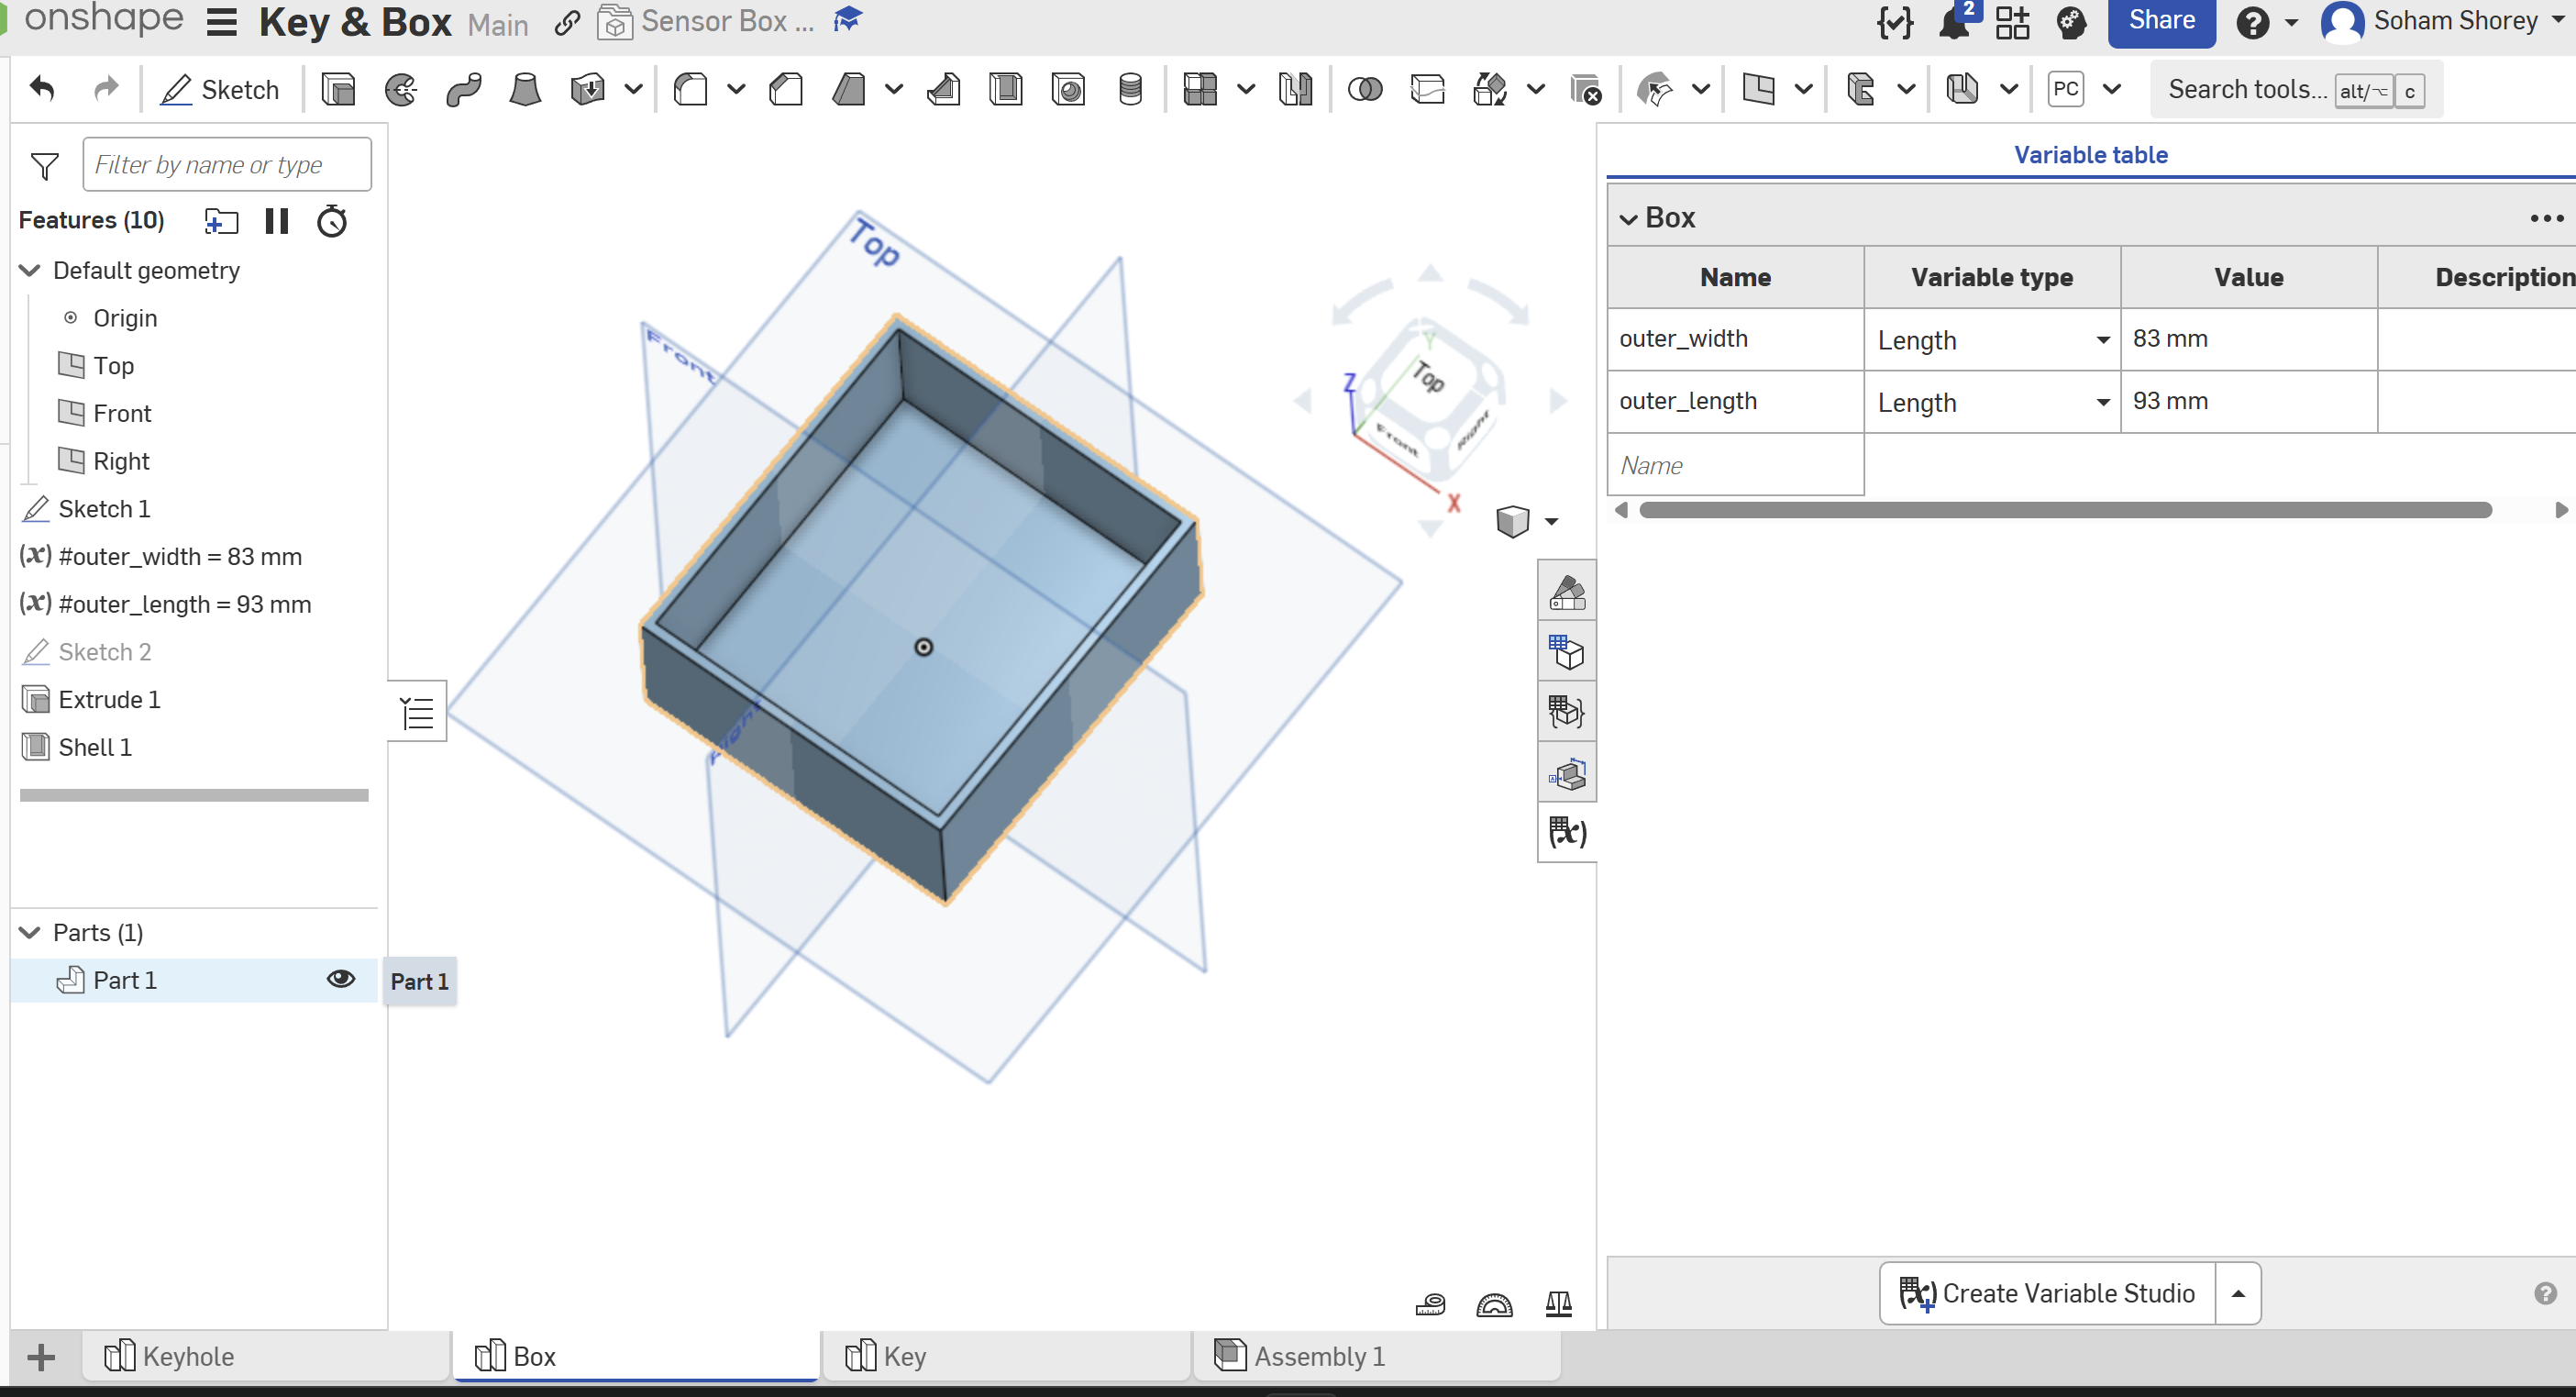
\includegraphics[width=0.70\textwidth]{images/initial_box_idea.png}
\caption{Initial CAD concept for the sensor box enclosure.}
\label{fig:initial_box}
\end{figure}

\subsection{Slidable Lid}

With the box body defined, a lid was needed to close the enclosure and allow access to the electronics. The initial approach was a simple press-fit cover; however, this was found to be impractical for repeated field removal. The lid design was then revised to use a slide mechanism, where the lid runs along two parallel grooves on the top edges of the box side walls and is retained by the channel geometry alone without fasteners. This allows the lid to be removed and reinserted quickly without tools. Figure \ref{fig:slidable_lid} shows the initial press-fit cover concept.

\begin{figure}[H]
\centering
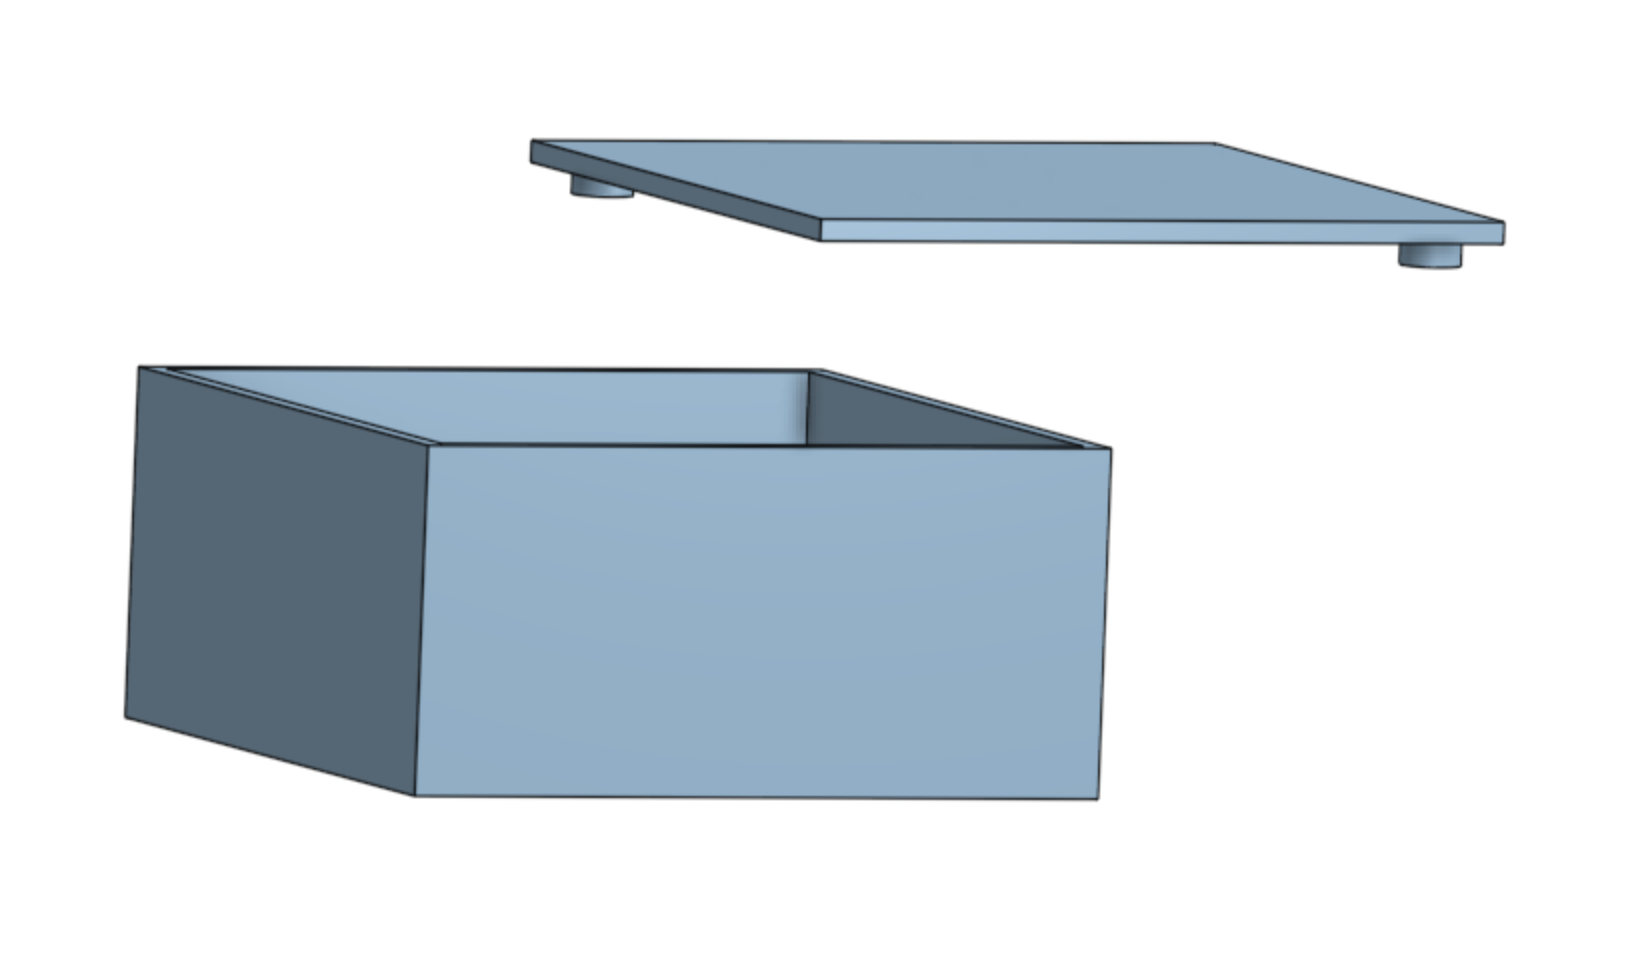
\includegraphics[width=0.70\textwidth]{images/slidable_lid_idea.png}
\caption{Initial press-fit cover concept for the sensor box enclosure.}
\label{fig:slidable_lid}
\end{figure}

\subsection{First Print and Tolerance Issue}

The box body and lid were printed in PLA using an FDM printer. The box body printed successfully; however, the lid could not be inserted into the grooves. The rail width on the lid was too wide to fit the groove on the box body. This was caused by a tolerance error in the CAD model where the groove and rail dimensions were specified as identical, without accounting for the dimensional expansion that occurs on closed features in FDM printing. Figure \ref{fig:lid_fit} shows the lid placed next to the box, where the mismatch is visible.

\begin{figure}[H]
\centering
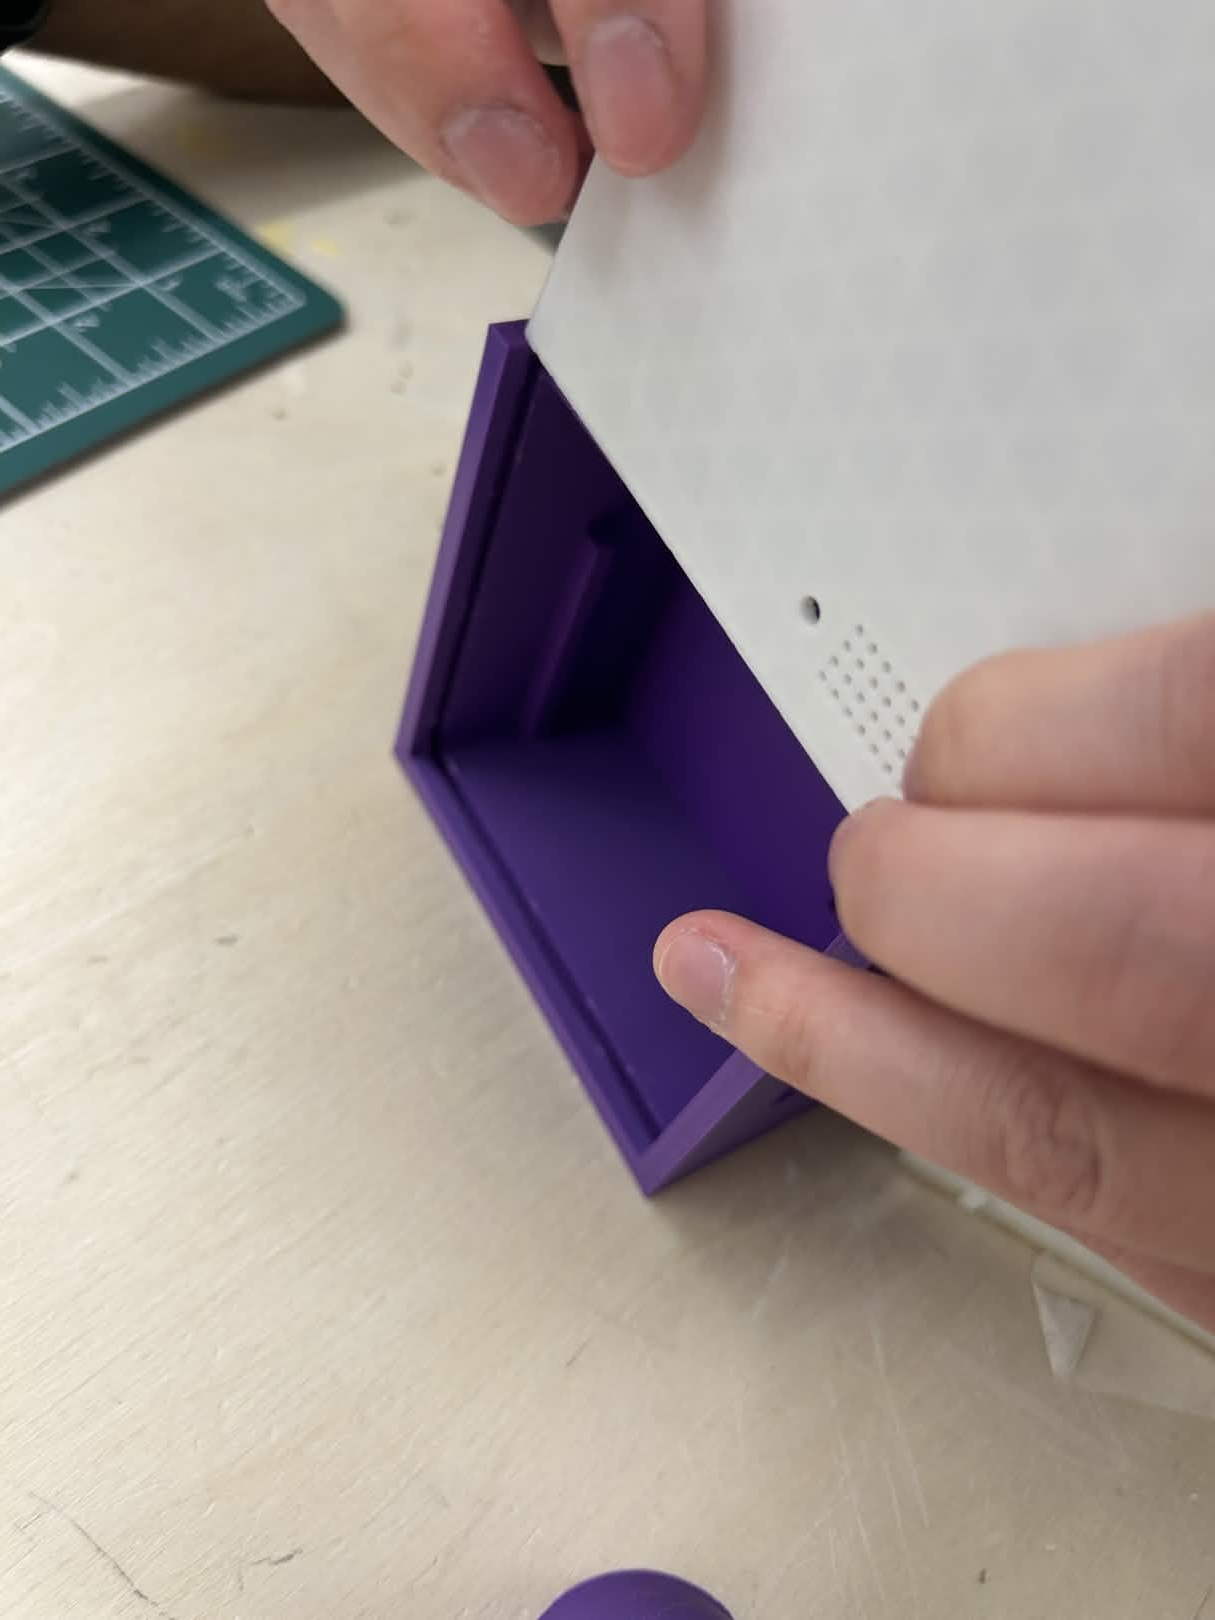
\includegraphics[width=0.70\textwidth]{images/Lid fits but needs sanding.jpg}
\caption{First-print lid next to the box body. The lid rail is too wide to enter the box groove.}
\label{fig:lid_fit}
\end{figure}

The planned correction is to update the CAD model with an appropriate clearance gap on the lid rail and reprint the lid. The box body does not require modification.

\section{Conclusion}

The rectangular sensor box and slidable lid design meet the requirements of compact electronics housing and tool-free field access. The first print confirmed the box body geometry but identified a tolerance error on the lid rail that prevented it from fitting the box groove. A CAD revision and lid reprint will resolve the issue.

\end{document}
